%% Copernicus Publications Manuscript Preparation Template for LaTeX Submissions
%% ---------------------------------
%% This template should be used for the following class files: copernicus.cls, copernicus2.cls, copernicus_discussions.cls
%% The class files, the Copernicus LaTeX Manual with detailed explanations regarding the comments
%% and some style files are bundled in the Copernicus Latex Package which can be downloaded from the different journal webpages.
%% For further assistance please contact the Publication Production Office (production@copernicus.org).
%% http://publications.copernicus.org


%% Differing comments regarding the specific class files are highlighted.


%% copernicus.cls
\documentclass[acp]{copernicus}

%% copernicus2.cls
%\documentclass[acp]{copernicus2}

%% copernicus_discussions.cls
%\documentclass[journal abbreviation, hvmath, online]{copernicus_discussions}

\usepackage[table]{xcolor}

\begin{document}


\title{Statistical analysis of an LES shallow cumulus cloud ensemble using a 
cloud tracking algorithm}


\author[1]{Jordan T Dawe}
\author[1]{Philip H Austin}

\affil[1]{Department of Earth and Ocean Sciences, 
        University of British Columbia, 
	6339 Stores Road, 
        Vancouver, BC, 
        V6T 1Z4}

%% The [] brackets identify the author to the corresponding affiliation, 1, 2, 3, etc. should be inserted.



\runningtitle{CLOUD TRACKING}

\runningauthor{Dawe and Austin}

\correspondence{Jordan T Dawe\\ (jdawe@eos.ubc.ca)}



\received{}
\pubdiscuss{} %% only important for two-stage journals
\revised{}
\accepted{}
\published{}

%% These dates will be inserted by the Publication Production Office during the typesetting process.


\firstpage{1}

\maketitle



\begin{abstract}
A technique for the tracking of individual clouds in a Large Eddy Simulation 
(LES) is presented.  We use this technique on an LES of a shallow cumulus cloud 
field based upon the Barbados Oceanographic and Meteorological Experiment 
(BOMEX) to calculate statistics of cloud height, lifetime, and other physical 
properties for individual clouds in the model.  We also examine the question of 
nature versus nurture in shallow cumulus clouds: do properties at cloud base 
determine the upper-level properties of the clouds (nature), or are cloud 
properties determined by the environmental conditions they encounter (nurture). 
We find that clouds which ascend through an environment that has been 
pre-moistened by previous cloud activity are no more likely to reach the 
inversion than clouds that ascend through a drier environment.  Cloud base 
thermodynamic properties are uncorrelated with upper-level cloud properties, 
while mean fractional entrainment and detrainment rate displays moderate 
correlations with cloud properties up to the inversion.  Conversely, cloud base 
area correlates well with upper-level cloud area and maximum cloud height.  We 
conclude that cloud thermodynamic properties are primarily influenced by 
entrainment and detrainment processes, cloud area and height are primarily 
influenced by cloud base area, and thus nature and nurture both play roles in 
the dynamics of BOMEX shallow cumulus clouds.
\end{abstract}

%% only used for copernicus2.clsu
%\abstract{
% TEXT
% \keywords{TEXT}}

\introduction
%% \introduction[modified heading if necessary]

Shallow cumulus clouds occur over large parts of the trade-wind regions 
\citep{Norris1988}, where subsiding air creates stable atmospheric conditions.  
They form an important part of the tropical Hadley circulation, acting to 
transport heat and moisture away from the surface, erode the inversion, and 
precondition the free troposphere for deep convection \citep{Tiedtke1988, 
Neggers2007}.  Additionally, since short-wave radiation reflection from marine 
boundary-layer clouds is a primary component of cloud radiative effects, a
proper parametrization of shallow cumulus is necessary to accurately model 
the global radiation balance in General Circulation Models 
\citep[GCMs;][]{Bony2005, Medeiros2008, Wyant2009, Medeiros2011}.

Much effort has been devoted to understanding the dynamics of shallow cumulus, 
notably the work of the Global Energy and Water Cycle Experiment (GEWEX) Cloud 
System Studies \citep[GCSS;][]{Randall2003} boundary layer cloud group.  The 
GCSS have created several idealized test cases, based upon field campaigns, 
suitable for modelling via Large Eddy Simulation \citep[LES;][]{Siebesma1995, 
Stevens2001, Brown2002, vanZanten2011}.  These studies have 
generally examined cloud fields in bulk, taking large-scale conditionally 
sampled mean values of quantities and fluxes.  This approach provides 
information about the mean cloud field properties, but averages out any 
information concerning the dynamics of individual clouds.

A few researchers have focused instead on simulating the dynamics of individual
clouds. Early work by \cite{Klaassen1985}, \cite{Bretherton1989} and 
\cite{Grabowski1991} performed two-dimensional simulations of a single 
cloud.  These were quickly followed by fully three-dimensional simulations 
\citep{Grabowski1993, Grabowski1993a, Carpenter1998, Blyth2005}, which 
simulated individual clouds initiated via the application of localized heat 
fluxes.  Unfortunately, none of these studies were able to examine how 
individual clouds might be affected by the presence of many other clouds in a 
cloud field.  To address this \cite{Zhao2005, Zhao2005a} manually selected six 
clouds from a fully-developed LES cloud field and analyzed their life cycles.  
A similar approach was taken by \cite{Heus2009}, who used a virtual-reality 
environment to help select 79 clouds from a set of LES experiments.

While the methods of \citeauthor{Zhao2005} and \citeauthor{Heus2009} were 
able to provide many insights into the dynamics of individual clouds in an 
LES cloud field, they still suffer from two issues.  First, they are time 
consuming, requiring human intervention to select individual clouds out of 
the model simulations, and second, they do not allow for a complete 
decomposition of a cloud field into individual clouds.  Ideally one would 
prefer an automated system that would be able to identify all individual clouds 
in an LES simulation and track them through their life history.

Two previous studies have looked at automated cloud identification and tracking 
in LES. \cite{Jiang2006} used a two-dimensional image registration algorithm 
to measure the effect of aerosols upon cloud lifetimes (Graham Feingold, 
personal communication, 2011).  This method of tracking projects the cloud 
liquid water path of individual cumuli onto a two-dimensional surface and 
tracks each entity over its lifetime. It has the benefit of simplicity, but is 
not appropriate for clouds that overlap in the vertical.  More recently, 
\cite{Plant2009} presented a tracking algorithm that was able to capture the 
complete time evolution of each cloud in an Cloud Resolving Model (CRM). This 
algorithm operates while the CRM is running, examines cloud relationships at 
each time step of the CRM, and outputs diagnostics for each individual cloud.

Here we present a fully automated algorithm for the tracking of individual 
clouds in an LES. This algorithm generates output similar to the algorithm 
created by \cite{Plant2009}, but with one significant difference: it can be 
run off-line, on pre-computed LES model fields.  In section 2 we describe the 
BOMEX LES we analyzed.  Section 3 presents the cloud tracking algorithm itself, 
and presents an overview of the statistics generated by the algorithm to compare 
the algorithm with simpler measures of the cloud field population both to 
sanity check the algorithm and characterize how the algorithm modifies the 
cloud field statistics.  Then in section 4 we use the output generated by the
algorithm to address the question of whether initial cloud properties or the
environment encountered by the cloud is more important in determining the 
course of the cloud's life cycle.  In section 5 we present our conclusions.  In
addition, we include the full source code for our algorithm for use by the LES
modeling community, written in the Python programming language, as supplemental
material to this paper.

%==============================================================================

\section{Model Description}

All LES calculations in this paper were made using version 6.7 of the System 
for Atmospheric Modeling \citep[SAM;][]{Khairoutdinov2003}.  The model run 
configuration was the standard GCSS Barbados Oceanographic and Meteorological 
Experiment \citep[BOMEX;][]{Holland1973, Siebesma2003} setup.  BOMEX simulates 
an idealized non-precipitating steady-state trade-wind cumulus cloud field 
based on observations made over ocean near Barbados during June, 1969.  
Constant latent and sensible surface heat fluxes, and constant large-scale 
moisture advection, subsidence, and radiative forcings drive the model.  Cloud 
base begins at 500 m height with maximum cloud fraction reached at 600 m, and 
the base of the inversion is roughly at 1500 m.

The BOMEX run was performed on a 6.4 km x 6.4 km horizontal x 3.2 km vertical 
domain with 25 meter grid resolution in all directions and a one second time 
step.  The model was run for 6 hours of model time, and the first three hours 
of simulation were discarded as the model was still adjusting into steady 
state. During the run the model steadily emits a numerical tracer from the 
surface which decays exponentially over time with a one minute time constant.  
This tracer is used to implement the conditional sampling of 
\cite{Couvreux2010} in order to track cloud plumes in the dry sub-cloud 
layer.  Model fields were output every minute for the last three hours of the 
simulation.

%==============================================================================

\section{Cloud Tracking}

Dividing a cloud field up into individual clouds at a single moment in time is 
a trivial matter of finding connected cloudy regions.  Tracking the resulting 
clouds from one time step to the next is more problematic, however.  The 
simplest possible algorithm would identify contiguous cloudy regions at each 
time step with unique ids, and then identify regions that overlap spatially in 
successive time steps, perhaps corrected for the effects of advection. This 
information could then be used to construct a graph of the cloud overlaps, and 
connected regions of this graph would represent individual tracked clouds.

However, when this simple algorithm is applied to the BOMEX cloud field the 
resulting graph is dominated by a small number (less than 10) of highly 
connected clouds that occupy over half the cloud field volume at any given time 
(not shown).  Futhermore, the resulting tracked clouds are not spatially 
localised--parts of individual tracked clouds may be on opposite sides of the 
domain. This result occurs because fleeting spatial connections between two 
clouds will result in those clouds belonging to a single connected cloud graph, 
no matter how long since they have been connected or how brief the connection.  

A cloud is a process, not an object; A rising parcel of moist air may condense, 
a parcel of air containing condensate may evaporate, and a cloud may merge with another cloud or split into multiple clouds.  To handle all of these possible 
events, we have developed a more complex method for tracking clouds in time.

\subsection{Cloud Tracking Algorithm}

In this section we present a description of our cloud tracking algorithm.  The 
major problem that our algorithm needs to solve is exactly how clouds should 
merge and split.  Our strategy to address this is to split each cloud into 
smaller regions, which we refer to as ``cloudlets'', formed around the buoyant 
cores of the clouds.  By deciding how to associate these cloudlets to clouds 
from the previous time step, tracked clouds are allowed to split and merge. A 
full implelemtation of our algorithm written in the Python programming language 
is included as supplemental material to this paper, and may be illustrative to
readers attempting to understand our technique.

We begin by defining three cloud regions (Fig. \ref{fig:vertical_section}).  
The first is the cloud ``core", defined following \cite{Siebesma1995} as all 
model points containing condensed liquid water which have positive buoyancy and 
upward velocity.  The second we refer to as the ``condensed" region, defined 
simply as all model points containing condensed liquid water.  Third is the 
cloud ``plume", the region of upward moving air that is associated with the 
cloud.  We define this region following the work of \cite{Couvreux2010} via a 
numerical tracer that is emitted at the surface and subsequently decays 
exponentially with a one minute time constant.  A point is considered to be in 
the plume if the tracer value of that point is larger than one standard 
deviation above the mean tracer value at the current height.  Additionally, 
the tracer value must exceed five percent of the mean of the horizontal 
standard deviation of the tracer values from the surface to the current height.  
However, unlike \citeauthor{Couvreux2010}, we do not require upper-level 
plume points to have condensed liquid water.  Finally, all condensed points are 
also flagged as plume points regardless of their tracer concentration, so that 
the condensed region is always a subset of the plume.

As mentioned above, at each time step we divide each model cloud into cloudlets 
formed around contiguous regions consisting of core grid points which are 
nearest-neighbour connected.  We do this by selecting a core gird point at 
random and assigning it a integer cloudlet id. Next, any core grid cells 
immediately above, below, north, south, east, and west of the initial core 
point are assigned the same cloudlet id.  This process is repeated recursively 
on these connected core points until all connected core points are assigned to 
the cloudlet.  Once this occurs, another core point which is not yet assigned a 
cloudlet id is chosen randomly, and the process is repeated until all core 
points are assigned to seperate cloudlets.

Next, condensed points are assigned to cloudlets in a process mimicing crystal 
growth, using the core points as cloudlet seeds. First we iterate through all
cloudlets created from the core regions, and assign condensed points that are
immediately nearest-neighbour connected to each cloudlet's points to the
cloudlet's id. Once a condensed point has a cloudlet id it is excluded from 
this process, so condensed points adjacent to more than one cloudlet's core are 
assigned to the cloudlet with the smalled id number.  This process is then 
repeated to assign ids to condensed points connected to the newly added 
cloudlet points, causing the cloudlets to grow into the condensed region until 
all connected condensed points are assigned to a cloudlet.  Leftover condensed 
points are then divided into new cloudlets via the same process used to assign 
core points to cloudlets.  Once all the condensed points have been assigned to
cloudlets, this expansion process is repeated for the plume points until all 
plume points are assigned a cloudlet id.  The entire cloudlet id assigning 
process is then repeated for every saved model time step.

This process of assigning plume, condensed, and core points to cloudlets 
results in condensed regions being divided into one or more cloudlets, each 
centered on contiguous core regions within the condensed region.  If a 
condensed region contains has no core points, the entire condensed region will 
be assigned to a single cloudlet.  This creates three types of cloudlets: ones
consisting of core points, surrounded by condensed points, surrounded by plume; 
ones consisting only of condensed points surrounded by plume; and ones 
consisting only of plume points. 

These cloudlets are then assigned integer tracking ids, which associate each 
cloudlet with a single tracked cloud.  For the first time step, we assign 
cloudlets which have nearest-neighbour connected condensed regions to the same
tracking id.  This causes the initial time step's clouds to be identical to 
those that would be identified simply by dividing the field up into connected 
regions of condensed liquid water.  At subsequent time steps, cloudlets that
spatially overlap with a tracked cloud at the previous time step are assumed to 
be the same tracked cloud.  The cloudlet's position is corrected for advection 
that has occurred between snapshots using the mean velocity of the cloudlet's
condensed points (if condensed points are present in the cloudlet) or plume (if 
they are not).

Four kinds of overlap are possible: condensed points in the cloudlet may 
overlap condensed points in a previous time step cloud 
(condensed$\rightarrow$condensed); condensed points may overlap previous 
plume points (plume$\rightarrow$condensed); plume may overlap condensed 
points (condensed$\rightarrow$plume); and plume may overlap plume 
(plume$\rightarrow$plume).  Several kinds of overlap may occur 
simultaneously, so we define a hierarchy of connection types and check each in 
turn.  The strongest connection type is condensed$\rightarrow$condensed, 
followed by plume$\rightarrow$condensed, then plume$\rightarrow$plume.  
Condensed$\rightarrow$plume connections are ignored, which prevents 
connections between newly formed cloudlets and leftover plume from a 
dissipating cloud.  Conversely, allowing plume$\rightarrow$condensed 
connections lets us associate newly condensed fluid with plumes rising through 
the sub-cloud layer.  Only the strongest connection type present for a given 
cloudlet is considered: if a cloudlet has condensed$\rightarrow$condensed 
connections, any condensed$\rightarrow$plume or plume$\rightarrow$plume 
connections are ignored, and if there are condensed$\rightarrow$plume 
connections, plume$\rightarrow$plume connections are ignored.  

Multiple overlaps between tracked clouds and cloudlets are used to identify 
merges and splits (Fig. \ref{fig:cloudfinder_instructions}).  Any cloudlet 
which overlaps more than one tracked cloud at the previous time step is 
considered to be the result of a merge between the tracked clouds.  In this 
case the cloudlet is assigned the tracking id of the cloud with the largest
overlap, and the other overlapping tracked clouds are assumed to have merged 
into the largest overlap cloud.  Next, tracked clouds that overlap more than 
one cloudlet are considered for splitting.  Splits occur only if a tracked 
cloud contains more than one cloudlet whose plume is in contact with the 
ground, with the largest cloudlet being assigned to the original cloud and the
smaller sub-clouds becoming new clouds. Cloudlets which are not connected to 
the ground are assigned to the nearest ground-connected cloud, measured by the
distance between the centroids of the cloud and cloudlet.  Any cloudlets that 
do not overlap clouds in the previous time step are assumed to be new clouds 
and are assigned new tracking ids. This process of cloudlet assignment, 
merging, splitting, and creation is repeated for each time step until all 
cloudlets are assigned tracking ids.
  
Next, any tracked cloud that has condensed points for less than five minutes is
flagged.  If any merge or split events occurred over these tracked clouds' 
short lifetimes, the tracked cloud is rejoined to the cloud it split from or 
merged into.  This prevents decaying detritus shed from a cloud top and clouds 
which split then immediately re-merge with their parent from being counted as
discrete cloud objects.  Finally, tracked clouds that have condensed liquid 
water only for a single time step are placed into a ``cloud noise" group. 

\subsection{Cloud Tracking Results}

Applying the cloud tracking algorithm to three hours of BOMEX LES output 
resulted in 3171 tracked clouds.  Of these, 609 (19\%) were created by 
splitting an existing cloud, 2381 (75\%) were unassociated with previous 
clouds, and 181 (6\%) were present at the start of the output period and thus 
their initiation was not observed.  Conversely, 261 (8\%) of the clouds ended 
their life cycle by merging with another cloud, 2820 (89\%) ended their 
life cycle by decaying away, and 90 (3\%) were present at the end of the output 
period.  A total of 850 clouds either begin by splitting from or end by merging 
with another cloud (27\%), indicating only 20 clouds both begin and end with 
such interactions (609 created via splitting, plus 261 destroyed via merging, 
minus 850, equals 20 which both split and merge).  The larger number of clouds 
present at the start of the output period (181) than at the end (90) is the 
result of the algorithm maintaining connections between physically separate 
clouds at the end of the output period.

Figure \ref{fig:example_cloud} displays horizontally averaged condensed region 
(cloud points containing condensed liquid water) properties for the 
longest-lived cloud in the ensemble.  The cloud's horizontal cross-sectional 
condensed area shows large, vertically coherent discontinuities in time due to 
merge events and split events.  However, the majority of the merge and split 
events that occur to this cloud do not significantly alter the cloud condensed 
area, and none of the other horizontally averaged properties display 
significant discontinuities.  Most of the cloud condensed region maintains 
upward velocities over 1 m s$^{-1}$ (Fig. \ref{fig:example_cloud}b), though 
short-lived downdrafts are apparent in the inversion (above $\approx$ 1.5 km) 
and at the end of the cloud's life.  Near cloud base, the total specific water 
($q_t$, units of g kg$^{-1}$, Fig. \ref{fig:example_cloud}c), liquid-water 
potential temperature ($\theta_l$, units of K, Fig. 
\ref{fig:example_cloud}d), and condensed liquid water ($q_l$, units of 
g kg$^{-1}$, Fig. \ref{fig:example_cloud}e) are similar to the mean 
environmental properties, but the $q_t$ excess, $\theta_l$ deficit, and 
$q_l$ of the condensed region increases with height, and indications of upward 
propagating pulses can be seen in these fields.  The condensed region buoyancy 
is generally positive below the inversion, with strong pulses of positive 
buoyancy apparent (displayed using density potential temperature 
$\theta_\rho$, units of K, Fig. \ref{fig:example_cloud}f).  Finally, 
comparing this example cloud with the example clouds presented by 
\citet[][figs. 4 and 5]{Heus2009} shows similar magnitudes and patterns in 
condensed region properties.

Core region (cloud points having upward velocity and positive buoyancy) 
properties for the same cloud (Fig. \ref{fig:example_core}) display buoyant 
mass pulses more clearly than the condensed region.  Cloud core occupies 
roughly 60\% the horizontal cloud area near cloud base, but essentially 
vanishes in the inversion.  Since the condensed region properties show positive 
vertical velocity and negative buoyancy in the inversion, the disappearance of 
the core must be due to the rapid increase of environmental stability, which 
makes the cloud negatively buoyant.  Cloud core vertical velocity increases 
steadily with height and $q_t$ excess, $\theta_l$ deficit, and $q_l$ are all 
greatest at cloud top.  Core buoyancy is positive by definition, and regular 
buoyant pulses are apparent.

The total BOMEX cloud fraction at cloud base in our model is about 0.065, or 
$\approx$ 2.7x10$^6$ m$^2$. The longest-lived cloud thus represents over 10\% 
of the total cloud base area at times.  As we mention at the beginning of this 
section, this is actually much smaller than the largest cloud tracked by a 
simple overlap algorithm that does not allow clouds to split and merge.  The 
dominance of the cloud field by this cloud is a natural outcome of the power
law distribution that shallow cumulus cloud areas are known to obey, since 
a power law implies the existance of a small number of extremely large clouds.

\subsection{Tracked Cloud Statistics}

In this section we examine the statistics of the cloud population generated by 
the tracking algorithm in order to sanity check the algorithm results, and to 
identify how and where the algorithm artificially modifies cloud field size
statistics.  Before calculating these statistics, we exclude any clouds which 
begin or end outside the model output period since we do not have access to 
their complete life cycles. This removes 287 clouds from the sample, leaving 
2,921.  This filtering will tend to preferentially affect the longest-lived 
clouds from our sample, biasing the population slightly.  However, our results 
show the cloud population to be overwhelmingly composed of short-lived clouds,
implying that robust statistics for the longest-lived clouds would not be 
possible with this three hour model run.

Both cloud lifetime (defined by the length of time the tracked cloud contains 
condensed points, Fig \ref{fig:cloud_stats}a) and mean condensed region mass 
over the cloud's lifetime (Fig \ref{fig:cloud_stats}b) are heavily skewed 
toward small, short-lived clouds.  The cloud lifetime distribution displays no 
clouds with a lifetime shorter than two minutes, due to our imposed constraint 
that tracked clouds be present at more than one model output time.  Over 1,000 
of the tracked clouds, a little less than a third of the total cloud 
population, exist for less than 4 minutes, and over 2,200 clouds, or about a 
half of the cloud population, have an average mass less than 10$^6$ kg 
($\approx$ 53 model grid cells).  Conversely, there are four clouds that 
persist for longer than an hour (not shown), and 35 with mean mass larger than 
3x10$^7$ kg ($\approx$ 1600 model grid cells, not shown).  Maximum cloud 
top height is much less skewed (skew = 2.0) than lifetime (3.6) and mass 
(10.4), but still shows many more small clouds than large clouds (Fig. 
\ref{fig:cloud_stats}c).  Only 441 clouds, or about 15\% of the population, 
reach a height of 1 km, and only 108 clouds (4\%) reach the inversion base at 
1.5 km.  Over 78\% of the clouds have cloud base between 500 and 600 m, with 
the majority of the rest having cloud base values below 1 km (Fig. 
\ref{fig:cloud_stats}d).  Thus, the overall picture of the cloud field we form 
is of numerous small, short-lived clouds at cloud base in a field dominated by 
a few large, long-lived towers that have managed to overcome convective 
inhibition and reach the inversion.

As cloud size distributions have been shown to be consistent with power law 
scalings \citep{Benner1998, Zhao2007}, these results are physically plausible. 
However, few of these statistics have been accurately measured in real cloud 
fields. One cloud property that has been widely measured, however, is 
horizontal cloud area taken from satellite and aircraft images 
\citep{Benner1998, Cahalan1989, Neggers2003, Neggers2003a, Zhao2007, 
Jiang2008}.  The number of clouds of a given size has been found to follow a 
power-law distribution of the form:
\begin{equation}
n(l) \propto l^{-\lambda}
\end{equation}
where $l$ is a horizontal length scale in meters generated by taking 
$l=\sqrt{a}$, $a$ is the horizontal area of the cloud, and $n(l)dl$ is the 
number of clouds with length scales between $l$ and $l+dl$.  $\lambda$ can 
be calculated by finding the slope of a line fit to a log-log plot of the 
relative number of clouds present at each length scale $l$.  Often this 
relationship is complicated by a scale break near $l$ = 1000 m, and so two 
power laws are fit, one for clouds with $l$ smaller than $\approx$ 1000 m and 
another for clouds with $l$ larger than $\approx$ 1000 m.

To calculate the cloud size distribution, we follow \cite{Neggers2003} and 
take the projection of the clouds' condensed regions onto a horizontal plane. 
This simulates what a satellite directly overhead would observe, to facilitate 
comparison with observations.  We then take the square root of the projected 
cloud condensed area to generate a length scale, calculate a cloud size 
histogram with 10 meter wide bins at each minute over the three hours of model 
output, then fit a line to this distribution in log-log space.  We do this 
twice, once for cloud sizes produced by the tracking algorithm, and once using 
cloud condensed region areas taken directly from snapshots of the model output.

Comparing the size distribution generated from snapshots with the distribution 
generated by the tracking algorithm shows the tracking algorithm modifies
the cloud size distribution by increasing the number of clouds between 100 and 
1000 m length scales, and removing clouds smaller and larger than this range 
(Figure \ref{fig:cloud_areas}).  The algorithm removes small clouds for two 
reasons: first, we explicitly filter out clouds that are present in only one 
snapshot; and second, the tracking algorithm treats short-lived clouds which 
have recently separated from a parent as part of the parent cloud.  Large
clouds are underrepresented by the algorithm for two reasons: first, clouds 
which have connected condensed regions may still have separate cores, and so 
are considered separate clouds by the algorithm; and second, the projection of 
the three dimensional cloud area onto the 2D plane done for the instantaneous 
snapshots results in clouds which overlap in the vertical, but which are 
disconnected in 3D space, inflating the numbers of large clouds seen in the 
snapshots.  Many of the small and large clouds thus end up classified as mid-
sized clouds by the tracking algorithm, inflating their numbers.

Clear scale breaks appear around 1000 m in the snapshot distribution and 900 m 
in the tracking algorithm distribution, and so we exclude length scales greater 
than 1000m and 900 m from the line fits used to find $\lambda$.  Additionally, 
a small-cloud scale break is apparent in the tracking algorithm distribution 
for clouds with $l$ less than 100 m, so we exclude this length scale from the 
tracking algorithm line fit as well.  Lines fit to the distributions result in 
reasonably similar values of $\lambda$: 1.88 for the snapshots, and 1.96 for 
the tracking algorithm (Figure \ref{fig:cloud_areas}).  These $\lambda$ 
values also compare favorably with previous estimates taken from LES 
(1.7, \citeauthor{Neggers2003},\citeyear{Neggers2003}; 1.9, 
\citeauthor{Jiang2008}, \citeyear{Jiang2008}), 
satellite observations (1.89, \citeauthor{Cahalan1989},
\citeyear{Cahalan1989}; 1.88, \citeauthor{Zhao2007}, \citeyear{Zhao2007})
and airplane observations (1.98, \citeauthor{Benner1998}, 
\citeyear{Benner1998}; 2.3, \citeauthor{Jiang2008}, \citeyear{Jiang2008}).
Thus, while the tracking algorithm modifies the total numbers of small, medium, 
and large clouds in the distribution, the power law scaling for the medium 
clouds is not significantly distorted.

%==============================================================================

\section{Two example analyses}

The output of the tracking algorithm provides us with a complete decomposition 
of the model cloud field into individual clouds.  This allows us to generate 
statistics of cloud behaviour and use these statistics to answer questions 
about cloud field dynamics.  Here we present two examples of analyses that 
would not be possible without a large database of tracked clouds.

Before we turn to our examples, we briefly examine the variability of the 
clouds in the tracked ensemble.  We examine six basic properties of the 
clouds' condensed liquid water regions: total specific water $q_t$, 
liquid-water potential temperature $\theta_l$, density potential temperature 
$\theta_\rho$, vertical velocity $w$, horizontal cross-sectional area $a$, 
and vertical mass flux $M$.  We take horizontal averages of the first four 
properties and horizontal sums for $a$ and $M$ over condensed points to 
generate property profiles for each cloud at each sampled time.

Correlations between the horizontal mean properties of all clouds present at a 
given height reveal strong relationships between the mean cloud properties 
(Figure \ref{fig:cloud_autocorrelation}).  Nearly identical results are found 
taking correlations of core properties, and so these results are applicable 
both to condensed and core regions.  Above 800 m, $q_t$, $-\theta_l$, and 
$\theta_\rho$ are strongly correlated, to the point that they can essentially 
be considered a single variable; more buoyant clouds have higher $q_t$ and 
lower $\theta_l$.  Similarly, $a$ and $M$ have near-unity correlations from 
600-1400 m, indicating that variations in horizontal cross-sectional area 
completely control the vertical mass flux.  From this we conclude that BOMEX 
cloud variability between 800 m and the inversion base can be completely 
characterized by three variables: $\theta_\rho$, $w$, and $a$.

Near cloud base the system becomes slightly more complicated, as $a$ and $M$ 
become uncorrelated and $-\theta_l$ diverges from $q_t$ and $\theta_\rho$.  
Below 600 m, buoyancy is controlled by variations in $q_t$, and $-\theta_l$ 
becomes anti-correlated with both $q_t$ and $\theta_\rho$, reaching a 
correlation of $\approx$ -0.9 at 500 m (not shown).  Within the 700-1400 m 
layer cross-correlations are significant at the 99\% confidence level between 
$\theta_\rho$, $w$, and $a$, but the magnitude of these relationships is much 
weaker, with a correlation of $\approx$ 0.75 between $w$ and $\theta_\rho$, 
$\approx$ 0.4 between $a$ and $\theta_\rho$, and $\approx$ 0.4 between $w$ 
and $a$.  Once the clouds reach the inversion layer, these correlations between 
$w$, $\theta_\rho$ and $a$ are no longer statistically significant.

Some of the causes of these cloud property cross-correlation patterns can be 
inferred from the vertical structure of the mean cloud condensed region 
properties (Figure \ref{fig:mean_profiles}).  All the BOMEX clouds begin with 
a small range of thermodynamic properties (relative to their mean values) at 
cloud base. The thermodynamic properties are then modified by mixing events as 
the clouds rise, resulting in accumulating variability that is strongly 
correlated.  Conversely, the BOMEX clouds start with a wide range of areas at 
cloud base, and as they rise this variation only grows a little.  Finally, the 
clouds start with some variability in their vertical velocity at cloud base, 
which increases as they rise due to variability in the buoyancy forcing.

Although $M$ is related to $a$ and $w$ via the relation $M = \rho w a$, where 
$\rho$ is the air density in kg m$^{-3}$, $M$ is only weakly correlated with 
$w$, despite being strongly correlated with $a$.  This unintuitive result 
arises due to the relative contributions of $a$ and $w$ to the variance of $M$.
Changes in $M$ can be expressed in terms of changes in $a$ and $w$ as
\begin{equation}
\label{eq:Mpartials}
d M = \rho w \partial {a} + \rho a \partial {w}
\end{equation}
Choosing representative cloud layer values into (\ref{eq:Mpartials}) is 
complicated by the power-law distribution that governs cloud areas.  The median 
values of $w$ and $a$ are roughly 0.5 m s$^{-1}$ and 10000 m$^2$ (Figure 
\ref{fig:mean_profiles}), while 66\% of $w$ and $a$ fall between roughly 
(0.1-1.0) m s$^{-1}$ and (1000-100000) m$^{2}$, respectively.  Differences in
cloud vertical velocity will thus result in mass flux values of approximately 
(1000-10000) kg s$^{-1}$, while differences in cloud cross-sectional area will 
results in mass flux values between (500-50000) kg s$^{-1}$, a range an order 
of magnitude larger.  Thus, cloud mass fluxes are primarily controlled by the 
area of the cloud, producing near unity correlations between $a$ and $M$.

Adopting the language of \cite{Romps2010a}, these results suggest that cloud 
area and mass flux results from the cloud's nature (initial conditions), and 
thermodynamic variables are governed by nurture (the environmental conditions 
they experience).  We examine this question further in the next section.

\subsection{Nature versus Nurture}

In this section, we perform analyses on the tracking algorithm output to 
address the question of nature versus nurture in shallow cumulus cloud 
dynamics: do the properties of the air entering the cloud at cloud base, or the 
properties of the environment the cloud encounters as it rises, exert stronger 
influence on the evolution of the cloud?  \cite{Romps2010a} addressed this 
question for individual parcels of convecting air and found the net entrainment 
experienced by a parcel influences the parcel's state far more than the 
parcel's initial properties at cloud base.  Our tracking algorithm allows us to 
examine this question from the prospective of whole clouds, instead of 
sub-cloud parcels.

We use a simple one-dimensional particle tracking model to examine the causes 
of variability in upper-level cloud properties.  For each cloud, we release a 
particle once a minute at some initial height and advect it vertically using 
the average vertical profile of $w$ in the cloud.  Linear interpolation is 
used to calculate $w$ between model grid points and sampling times, and forward 
differencing is used to step the particle position in time with a time step of 
1 s.  The times at which the particles reach each higher model level are then 
recorded until the particle leaves the cloud (Figure 
\ref{fig:cloud_base_schematic}a).  

These time-height profiles are then used to sample the mean properties of the 
cloud when the released particles reach each model level (Figure 
\ref{fig:cloud_base_schematic}b and c).  We then combine the results from each 
cloud in the simulation to produce correlations between the cloud properties 
when the particles are released and when they reach each model height (Figure 
\ref{fig:cloud_base_schematic}d).  If a particle does not reach a given 
height, it is simply excluded from the correlation calculation.  This allows us 
to determine to what extent the properties of the cloud near cloud base control 
the future properties of the cloud at height.

We use the 99\% significance level as a rough measure of the height at which 
the cloud properties are decorrelated from the properties at particle release.  
However, since clouds tend to experience discrete mass flux pulses on a 
$\approx$ 15 minute timescale and we release one particle each minute, we 
divide the degrees of freedom (number of particles) used to calculate the 
correlation significance by a factor of 15 to account for the auto-correlation 
of cloud properties within a pulse.

First, we perform this calculation using particles released from a height of 
300 m, in the sub-cloud layer.  Since condensed liquid water does not appear in 
the sub-cloud layer, we use the horizontal mean properties of the cloud plume 
region to advect the particles and calculate property values.  A total of 8012 
particles are released at 300 m and tracked.  For this calculation we ignore 
plume area and vertical mass flux, because the method we use to divide the 
sub-cloud plume up between individual clouds makes the area of the sub-cloud 
plume dependent on that of the cloud core above.

The $q_t$ of the rising particles is strongly correlated with $q_t$ at release 
up until the particles reach cloud base at 500 m (Figure 
\ref{fig:sub_cloud_profiles}).  The mean $\theta_l$ and $\theta_\rho$ of 
the plume are also strongly correlated with release properties.  This implies 
that the sub-cloud plume properties propagate upward essentially unchanged by 
interaction with surrounding air.  $q_t$ is anti-correlated with $\theta_l$ 
with a value of $\approx$ 0.6 in the sub-cloud layer, and does not show 
significant correlations with $\theta_\rho$.  Conversely, $\theta_\rho$ is 
strongly correlated with $\theta_l$ but not with $q_t$; thus, while in the 
cloud-layer buoyancy is controlled by $q_t$, in the sub-cloud layer, it is 
controlled by $\theta_l$.  The $w$ of the rising particles is uncorrelated 
with any other properties at particle release with the exception of the 
velocity, but unlike the thermodynamic variables this correlation steadily 
declines and become insignificant 200 m above the particle release level, 
indicating the vertical velocity is strongly modified in the sub-cloud layer.  
The transition from the sub-cloud layer into cloud base fully decorrelates the 
$w$ and $\theta_\rho$ of the cloud with the sub-cloud properties at 300 m.
Only $q_t$ and $\theta_l$ properties survive the transit through cloud base, 
but the correlation with the sub-cloud properties is limited to the first 200 m 
above cloud base.

Next we look at correlations profiles for particles released at 600 m, the 
height of maximum cloud fraction in the middle of the cloud base layer.
For this height we use the horizontal mean of the cloud core properties to 
advect the particles and calculate cloud properties, as the cloud core 
definition insures the particles will always move upward.  A total of 
9984 particles are released and tracked.  Due to the strong cross-correlations 
between thermodynamic variables and cloud area and mass flux, we restrict our 
analysis to $\theta_\rho$, $w$, and $a$.  However, since $\theta_l$ is 
uncorrelated with $q_t$ and $\theta_\rho$ at cloud base, we do calculate the 
correlation between $\theta_l$ at 600 m and upper-level properties separately 
from cloud base $\theta_\rho$.

Cloud base $\theta_l$ turns out to be uncorrelated with any upper-level 
cloud core properties (Figure \ref{fig:cloud_base_profiles}).  Correlations 
between $\theta_\rho$ at cloud base and at height decline rapidly, dropping 
below 0.5 by 800 m and losing all statistical significance around 1,000 m.  
Cloud base $w$ and $a$ are correlated with $\theta_\rho$ at cloud base at 
levels of 0.25 and 0.5, respectively, and this correlation also falls to 
insignificance by 1000 m.  Vertical velocity shows a similar pattern, with all 
correlations becoming insignificant near 1,000 m.  Cloud core area, on the 
other hand, is significantly correlated with cloud base area all the way up to 
the inversion base at 1,500 m.  Cloud base $w$ is also significantly correlated 
with upper-level cloud core area up to 1,300 m, but with a much smaller 
correlation.  In summary, upper-level thermodynamic properties and vertical 
velocity appear to be uncorrelated with cloud-base properties, but upper-level 
cloud core area is correlated with cloud base $a$ and, to a lesser extent, $w$.

\cite{Romps2010a} explained the variation in cloud parcel properties at height 
as the result of the entrainment the parcel experienced as it rose from 
cloud base.  We can examine the influence of entrainment and detrainment 
processes on the cloud core properties by taking the mean of the total 
fractional cloud core entrainment $\epsilon$ (in units of m$^{-1}$) and 
fractional cloud core detrainment $\delta$ (also in m$^{-1}$) experienced by 
the particle between 600 m and the current height, and correlating these
$\bar{\epsilon}$ and $\bar{\delta}$ values (where the over-bar denotes the 
mean of the property between cloud base and the current height) with the 
properties of the cloud core at the current height.  To do this we calculate 
cloud core mass entrainment and detrainment rate profiles for each individual 
cloud using the direct entrainment method detailed in \cite{Dawe2011}, and 
divide these profiles by the cloud core vertical mass flux of each cloud to 
generate individual $\epsilon$ and $\delta$ values for each cloud at each 
particle sampling time.  Additionally, we calculate the mean of the critical 
mixing fraction $\chi_c$, the fraction of environmental air in a mixture of 
core and environmental air needed to produce a neutrally buoyant mixture.  
$\chi_c$ is used in buoyancy-sorting parametrization schemes to determine 
cloud core entrainment and detrainment rates \citep{Kain1990, Rooy2008}.  We 
calculate $\chi_c$ using the mean cloud core properties and environmental 
properties taken as the average of all non-cloud core points at the current 
height within 100 m of the cloud core.

Cloud core $\theta_\rho$ is anti-correlated with $\bar{\epsilon}$ and 
$\bar{\delta}$, and correlated with $\bar{\chi_c}$, with a constant 
magnitude of roughly 0.5 up to 1,400 m (Figure 
\ref{fig:cloud_base_integrals_env}). These correlations become stronger than 
the correlation with cloud base $\theta\rho$ roughly 200 m above particle 
release, and indicate that low entrainment and detrainment rates are correlated 
with anomalously buoyant clouds.  Vertical velocity also shows stronger 
correlations with -$\bar{\epsilon}$, -$\bar{\delta}$, and $\bar{\chi_c}$ 
than with cloud base $w$ between 800-1,300 m, although in this case 
-$\bar{\delta}$ has a noticeably higher correlation with $w$ than 
-$\bar{\epsilon}$ does.  Conversely, cloud core area is more correlated with 
cloud base core area than -$\bar{\epsilon}$, -$\bar{\delta}$ or 
$\bar{\chi_c}$ all the way to the inversion base, at which point the 
-$\bar{\delta}$ and $\bar{\chi_c}$ values show roughly the same correlation 
with $a$ as cloud base area.  -$\bar{\epsilon}$ is far less 
correlated with $a$, however, showing that cloud area variations are more 
influenced by detrainment than entrainment.

Our results largely agree with the results of \cite{Romps2010a}: upper-level 
cloud properties are governed by the entrainment and detrainment experienced by 
the cloud as it rises, and cloud base properties have little influence on 
upper-level cloud properties, suggesting that nurture is more important than 
nature in determining shallow cumulus cloud properties.  The exception to this
is cloud area, which is correlated with cloud base area and which
\citeauthor{Romps2010a} were not able to examine with their parcel model.
Nevertheless, cloud base area and entrainment/detrainment rates still exert 
roughly equal influence over upper-level cloud area.

\subsection{Ascending cloud top properties versus maximum cloud height}

In this section, we examine the effect that the properties of the cloud top and 
the environment the cloud encounters as it ascends has upon the eventual height 
the cloud achieves.  Using the cloud tracking data, we identify the earliest 
times that condensed liquid water is present at each height during each cloud's 
ascent (Fig. \ref{fig:cloud_environment_schematic}a).  We then find all 
condensed points within 100 m of the cloud at those heights and time, and take 
averages of the properties of those points to generate vertical profiles of the 
ascending cloud top properties (Fig. \ref{fig:cloud_environment_schematic}b).  
Additionally, we find all environment points that are nearest-neighbour 
adjacent to the cloud top condensed points between 0 m and 50 m below cloud top 
and extend the topmost nearest-neighbour points 50 m above cloud top to 
generate profiles of the environment encountered by the rising cloud top.

From these profiles, we perform two analyses based upon the average of the 
property profiles between 550-750 m and between 750-1000 m.  In order to not 
bias these averages, any cloud profiles which do not span the whole averaging 
range are excluded from the analysis.  Clouds whose life histories begin or end 
outside the data period are also discarded.  From the original set of 3,171 
clouds, this leaves 257 clouds in the 550-750 m case and 240 clouds in the 
750-1000 m case.

The clouds that remain are then split into two categories: tall clouds which 
exceed a threshold height over their lifetime, and short clouds which do not.  
The threshold height is chosen in each case to divide the cloud sample roughly 
equally.  For the clouds present between 550-750 m, we set the dividing 
height to 1125 m; for the clouds present between 750-1000 m, we set the 
dividing height to 1300 m.  This results in 131 tall clouds and 136 short 
clouds in the 550-750 m case, and 127 tall and 113 short clouds in the 
750-1000 m case.

Since some of the cloud's properties, such as horizontal cross-sectional area, 
are not normally distributed, we use a non-parametric statistical test to 
determine if the properties of the tall clouds and their environment are 
significantly different than the properties of the short clouds.  The 
Mann-Whitney U test evaluates the null hypothesis that two data samples come 
from the same distribution \citep{Mann1947}.  It does this by summing the 
number of values in one sample which are greater than each value in the other 
sample; this sum is called $U$.  If large samples are taken from populations 
with identical distributions, on average one would expect a given value from 
the first sample to be larger than half the values in the other sample, and $U$ 
will be normally distributed with a mean value of $mn/2$.  Thus, the further 
$U$ is from $mn/2$, the more likely it is that the two samples come from 
distributions with differing magnitudes.  Note that there are actually two U 
values defined by this test, depending on whether the first sample is ranked 
against the second, or the second is ranked against the first.  However, it is 
easy to show that $U_1 + U_2 = mn$, and by convention only the smaller U-value 
is quoted.

We calculate U values for total specific water $q_t$, liquid-water potential 
temperature $\theta_l$, density potential temperature $\theta_\rho$, and 
vertical velocity $w$ for both cloud top and environment.  Three additional 
quantities are calculated for cloud top alone: specific liquid water $q_l$, 
horizontal cross sectional area $a$, and vertical mass flux $M$ (in units of 
kg s$^{-1}$).  All of these values are calculated for both averages over 
550-750 m and 750-1000 m, resulting in a total of 22 property comparisons.  
For the 550-750 m samples, if both the tall and short clouds have identical 
distributions the mean value of $U$ should be 8908, and for the 750-1000 m 
samples, 7175.  

Since we are calculating 22 separate tests, there is a high chance that one of 
these tests will show a spurious significant relationship if we test for a 95\% 
significance level.  Several methods, such as the Bonferonni correction 
\citep{Shaffer1995}, can be used to reduce the possibility of finding a 
spurious result.  However, these methods often risk erroneously excluding 
significant results, and much debate over their use can be found in the 
scientific literature \citep{Perneger1998, Nakagawa2004}.  The simplest 
correction to significance for multiple statistical tests is simply to divide 
the p-value sought by the number of tests performed.  Thus, to achieve an 
overall p-value of 0.05 with 22 tests, we must achieve a p-value of 0.05/22 = 
0.0023 on an individual test. This represents a worst case scenario where only 
one of the 22 tests is significant, and we must exclude the possibility this 
significance results from random chance; if more than one test is significant, 
the p-value needed to exclude false positives is reduced.  Instead of 
calculating these probabilities explicitly, we will simply consider any result 
with p \textless 0.05 as possibly significant and any with p \textless 
0.0023 as definitely significant.  

Our results are presented in Table 1.  We find that the environmental 
$q_t$, $\theta_l$ and $\theta_\rho$ encountered by the clouds between 
550-750 m are not significantly different for tall clouds than for short clouds.  
Environmental $w$ is on the borderline for statistical significance, with 
velocities on average 0.05 m s$^{-1}$ larger between 550-750 m for the tall 
clouds than the short clouds.  On the other hand, cloud top properties show 
strong differences between tall and short clouds, with only $\theta_l$ showing 
no differences.  Cloud top $\theta_\rho$ is possibly significant, with 
more buoyant clouds slightly more likely to become tall, but much more 
important are the cloud humidity, vertical velocity, and especially horizontal 
cloud cross-sectional area and mass flux, which have extremely small p-values 
of 2.2x10$^{-16}$ and 6.8x10$^{-21}$, respectively; moist clouds, rising 
quickly, with larger horizontal cross-sectional areas and greater vertical mass 
flux are more likely to become tall clouds.

However, simply because the differences in these values are statistically 
significant does not mean that they are important.  Examining histograms of 
environmental $w$ and cloud top $\theta_\rho$, $w$, and $a$ (Figure 
\ref{fig:cloud_environment_histograms}) shows that, while the differences 
between the tall and short clouds are unlikely to have occurred by chance, 
clouds tops with small areas, in relatively slowly rising environments, still 
have a reasonable chance of becoming tall clouds.  These properties certainly 
have an influence on the cloud height, but it is clearly not a definitive one.

As the clouds rise above cloud base, similar results appear for the properties
associated with short and tall clouds change (Table 1). None of the 
environmental properties encountered by the clouds between 750-1000 m are significantly different for short clouds than for tall clouds.  However, all 
tested cloud top variables show significant differences between the short and 
tall clouds.  Clouds with large $q_t$, $q_l$, $\theta_\rho$, $w$, $a$, and 
$M$, and lower $\theta_l$, between 750-1000 m, are more likely to rise past 
1300 m.  Of these properties, cloud top area and mass flux are again the most
significant differences.

\subsection{Discussion}

Our results present the following picture of the dynamics of the BOMEX cloud 
field.  The sub-cloud layer is well mixed and filled with broad regions of 
upward and downward motion (Figure \ref{fig:vertical_section}).  These regions 
are large enough that they are relatively shielded from mixing with other air 
masses and property anomalies easily propagate vertically.  Conversely, the 
mean upward velocity of plumes in this region is uncorrelated with the plume's 
mean buoyancy and plume velocity anomalies dissipate quickly as the plumes 
rise, suggesting the sub-cloud plume dynamics are dominated by inertia and 
pressure effects.

Once the broad regions of rising air reach cloud base, they enter a different 
physical regime.  As rising parcels reach the top of the sub-cloud layer they 
lose buoyancy, and must rely on inertia and pressure perturbations to 
allow them to continue rising.  Thus, the environmental stability at cloud base 
acts as a filter which admits only the fastest moving parcels, or the parcels 
in a region of organized motion with a pressure perturbation sufficient to 
overcome the negative buoyancy (i.e., a cloud with a large horizontal area).  
Hence, larger area clouds in an upward moving environment are better able to
penetrate through cloud base.

However, above the cloud base region there is a third regime.  The fate of 
clouds above the cloud base is determined by a race between the rate the cloud 
moves upward and the rate the cloud is mixed away into the environment.  As the 
clouds rise, latent heating from condensation enhances their buoyancy and 
creates a feedback loop in which faster moving clouds gain more buoyancy, and 
more buoyant clouds move faster.  At the same time, entrainment and mixing 
tend to wipe out this excess buoyancy.  Clouds with higher moisture content and 
buoyancy are more likely to remain buoyant, so thermodynamic quantities become 
important in determining eventual cloud height.  However, cloud area dominates 
these effects, as larger clouds are better able to shield their cores from 
mixing with the environment.  This process persists until the clouds reach the 
inversion, where the latent heating rate is incapable of keeping the clouds 
buoyant in the face of the strong $\theta$ gradient, and they are mixed 
away.

\cite{Neggers2002} construct a theory in which fractional entrainment rate 
is inversely proportional to vertical velocity and cloud parcels enter cloud 
base with a wide range of properties.  The variations in parcel properties then 
set the entrainment rate and thus control the future evolution of the parcel 
properties.  Our results disagree with the assumption of 
\citeauthor{Neggers2002} that parcels have a range of initial thermodynamic 
conditions.  We have not directly examined the dependance of entrainment rate 
on vertical velocity; however, the strong relationship between eventual height 
reached by the clouds and the cloud area suggests that fractional entrainment 
is more likely dependent on cloud area and any relationship between vertical 
velocity and entrainment is due to larger area clouds shielding their cores 
from entrainment, producing higher buoyancies and vertical velocities.

Using numerical tracers in a BOMEX LES, \cite{Romps2010a} found that 
stochastic entrainment controlled the evolution of convecting parcels, not 
the thermodynamic properties of those parcels at cloud base.  Our results 
extend this conclusion to apply to whole clouds.  However, our results also 
show that cloud base area exerts strong controls over the upper-level area and 
maximum height of the cloud.  Because of this we conclude that both nature, in 
the form of cloud base area, and nurture, in the form of entrainment and 
detrainment, have roles in the dynamics of BOMEX shallow cumulus clouds.  

Finally, the strong effect we find that cloud area has on the eventual cloud 
top height cloud suggests a simple physical interpretation for the stochastic 
entrainment event parametrization proposed by \cite{Romps2010a}: entrainment 
events occur when a parcel reaches the edge of the cloud.  This idea is 
supported by examining the changes in the probability distribution of $q_t$ 
values at various distances from the cloud surface (Figure 
\ref{fig:qt_vs_dist}): cloud parcels far from the cloud surface display higher
mean humidities than parcels near the cloud surface, indicating that interior 
parcels are shielded from mixing with the environment.  This hypothesis 
implies that the probability of a parcel experiencing an entrainment event 
should be related to the ratio of the total cloud area to the area of the 
cloud within some mixing length of the cloud edge.

%==============================================================================

\conclusions
%% \conclusions[modified heading if necessary]
We have developed an algorithm for tracking individual shallow cumulus clouds 
in an LES simulation which generates reasonable statistical distributions for a 
variety of cloud properties.  The key innovations this algorithm employs are 
the use of non-buoyant cloud parcels as a buffer region to mediate merging and 
splitting of buoyant cloud plumes, and a numerical tracer which we use to 
evaluate if a cloud plume remains dynamically connected to the surface layer.  
The output of this algorithm is suitable for conducting statistical 
analyses of shallow cumulus cloud populations.  We believe this algorithm could 
be easily extended to study deep convection.  We include in the supplementary 
material of this paper our implementation of this algorithm, written in Python, 
for general use by the cloud modeling community.

BOMEX cloud properties above cloud base divide into three categories of 
variables that are highly correlated within each category: the thermodynamic 
properties $q_t$, $\theta_l$, and $\theta_\rho$; the vertical velocity $w$; 
and the area $a$ and vertical mass flux $M$.  The thermodynamic properties show 
little variation at cloud base, but their variability increases steadily with 
height; cloud area is quite variable at cloud base and maintains its variance 
with height; and vertical velocity falls between these two extremes.

Analyzing the upward propagation of property anomalies shows three sets of 
processes operating on the clouds at different heights.  Below cloud base, 
cloud plumes are large and homogenous and upward motion is primarily governed 
by turbulence.  The buoyancy of plumes rapidly decreases at cloud base, which 
prevents all but the fastest rising plumes from penetrating into the cloud 
layer.  If these plumes make it through the cloud base layer, dilution by the 
environment competes with buoyancy production from latent heating to control 
the ascent of the clouds to the inversion.  These results suggest that 
nature controls the area and eventual height reached by the clouds, while 
nurture controls their thermodynamic properties.

%\appendix
%\section{\\ \\ \hspace*{-7mm} HEADING}    %% Appendix A

%\subsection                               %% Appendix A1, A2, etc.

\begin{acknowledgements}
Support for this research was provided by the Canadian Foundation for Climate 
and Atmospheric Science through the Cloud Aerosol Feedback and Climate 
network. We thank Marat Khairoutdinov for making SAM available to the cloud 
modeling community. Figures were generated using the matplotlib library in the 
Python programming language.
\end{acknowledgements}


\bibliographystyle{copernicus}
\bibliography{./bibliography/cloud_tracking}


%% Literature citations
%% command                        & example result
%% \citet{jones90}|               & Jones et al.\ (1990)
%% \citep{jones90}|               & (Jones et al., 1990)
%% \citep{jones90,jones93}|       & (Jones et al., 1990, 1993)
%% \citep[p.~32]{jones90}|        & (Jones et al., 1990, p.~32)
%% \citep[e.g.,][]{jones90}|      & (e.g., Jones et al., 1990)
%% \citep[e.g.,][p.~32]{jones90}| & (e.g., Jones et al., 1990, p.~32)
%% \citeauthor{jones90}|          & Jones et al.
%% \citeyear{jones90}|            & 1990






%% FIGURES %%%%%%%%%%%%%%%%%%%%%%%%%%%%%%%%%%%%%%%%%%%%%%%%%%%%%%%%%%%%%%%%%%%%


%% ONE-COLUMN FIGURES

%f
%\begin{figure}[t]
%\vspace*{2mm}
%\begin{center}
%\includegraphics[width=8.3cm]{./figures/figure1}
%\end{center}
%\caption{Schematic representation of our cloudlet algorithm.}
%\label{fig:cloudfinder_instructions}
%\end{figure}


%% TWO-COLUMN FIGURES

%f
\begin{figure*}[t]
\vspace*{2mm}
\begin{center}
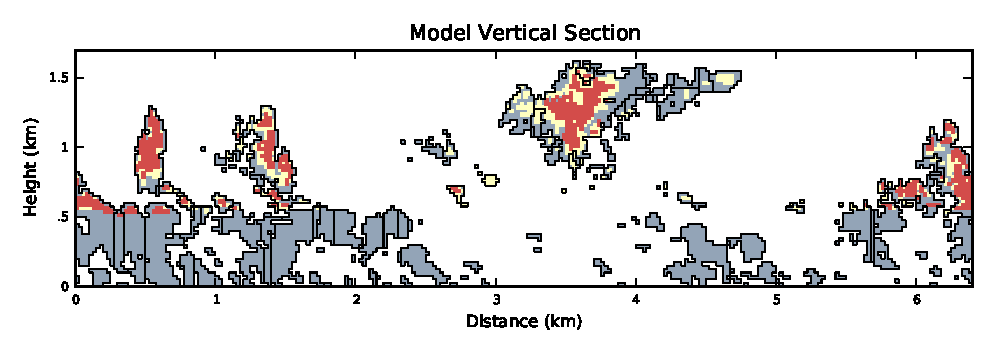
\includegraphics[width=\textwidth]{./figures/vertical_section}
\end{center}
\caption{Vertical section through the BOMEX model, showing the cloud core
(dark red), condensed liquid water (blue) and the plume (light yellow) regions 
used by the cloud tracking algorithm. Black lines show the edges of 
``cloudlets" identified by the cloud tracking algorithm.}
\label{fig:vertical_section}
\end{figure*}

%f
\begin{figure}[t]
\vspace*{2mm}
\begin{center}
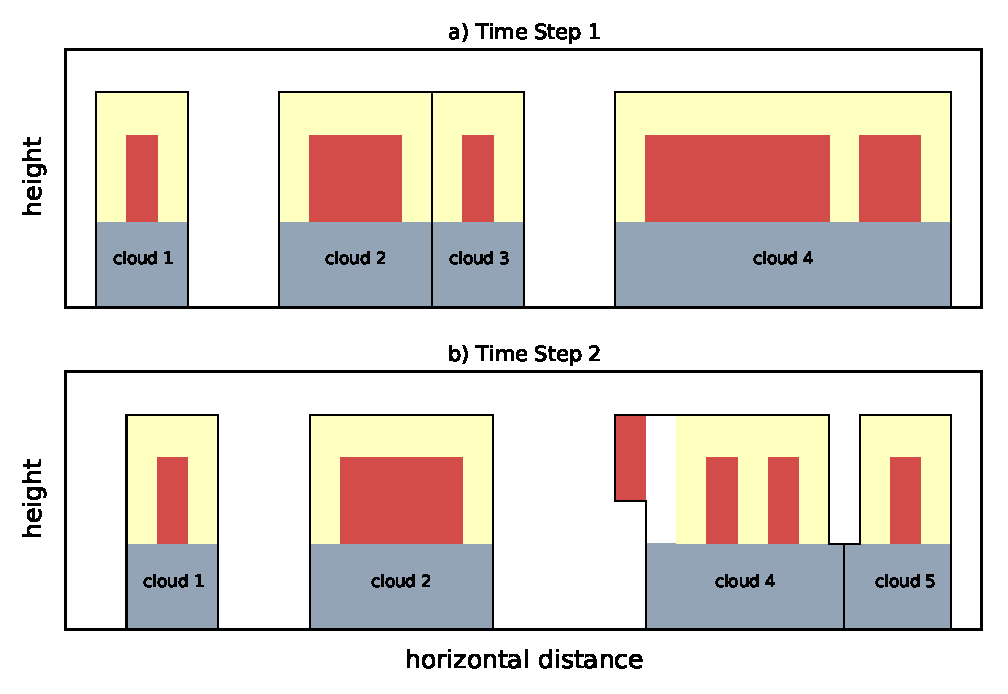
\includegraphics[width=8.3cm]{./figures/cloudfinder_instructions}
\end{center}
\caption{Example of possible relationships between clouds at two adjacent 
times.  Top panel represents a vertical model section showing 4 clouds being 
tracked by the algorithm. Bottom panel represents the same vertical model 
section 1 minute later. As in Figure 1, cloud core is dark red, condensed 
liquid water is blue, and the tracer plume is light yellow.  The left side of 
the sections shows cloud 1 tracked between time steps.  The middle of the 
sections shows two clouds merging; in the first time step, the clouds' 
condensed regions have come into contact, but not until their cores contact 
does cloud 3 merge into cloud 2. The right side of the sections shows a cloud 
splitting in two; cloud 5 splits from cloud 4 since their condensed regions 
have separated, while the disconnected core region on the left side of cloud 4 
has not separated since it is not connected to ground level by the cloud 
plume.}
\label{fig:cloudfinder_instructions}
\end{figure}

%f
\begin{figure*}[t]
\vspace*{2mm}
\begin{center}
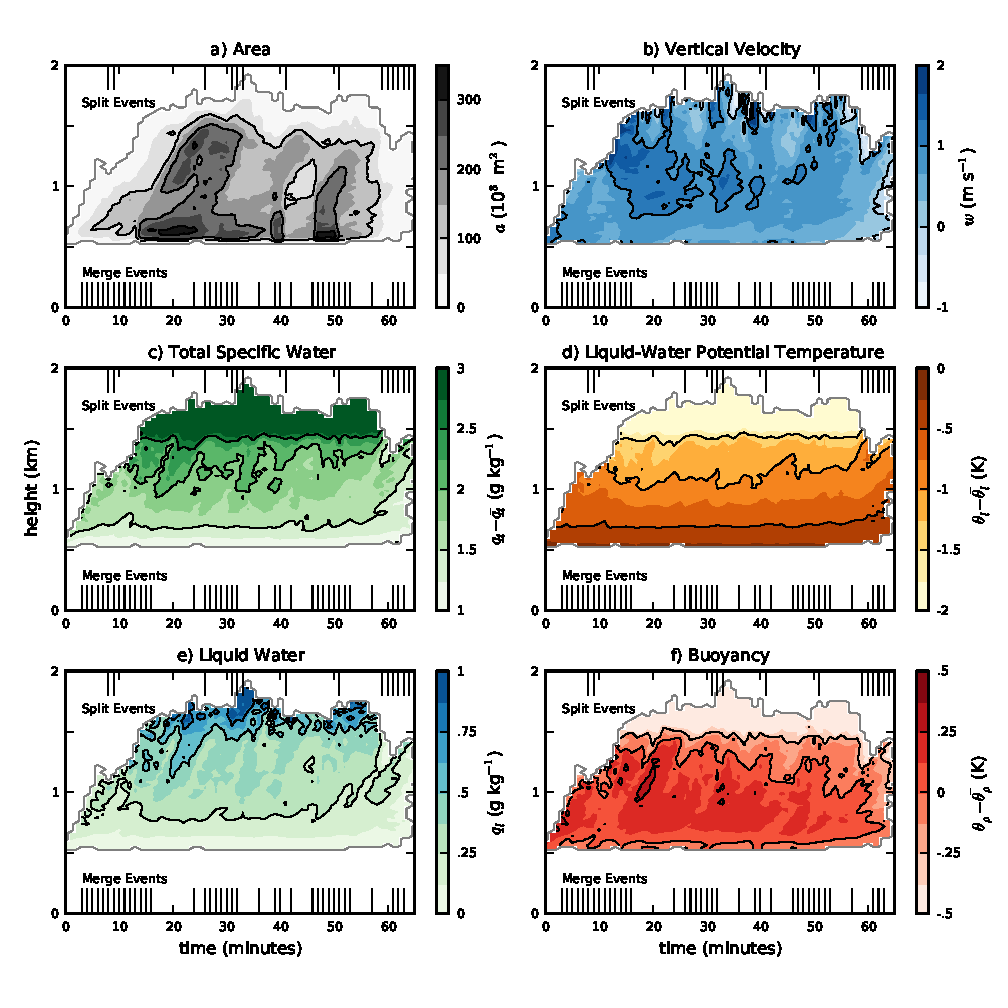
\includegraphics[width=\textwidth]{./figures/example_cloud}
\end{center}
\caption{Height-time profiles of a) horizontal cross-sectional area, 
b) vertical velocity, c) total specific water surplus, d) liquid-water 
potential temperature deficit, e) specific liquid water and f) buoyancy of the 
condensed liquid water region of the longest-lived tracked cloud.  Surplus and 
deficit values in c) and d) are relative to the horizontal mean properties of 
the model.  The black lines in b) and f) denote the zero contours.  The longer 
line markers at the top and bottom of the plots denote the times at which 
clouds split from and merge into this cloud, respectively.}
\label{fig:example_cloud}
\end{figure*}

%f
\begin{figure*}[t]
\vspace*{2mm}
\begin{center}
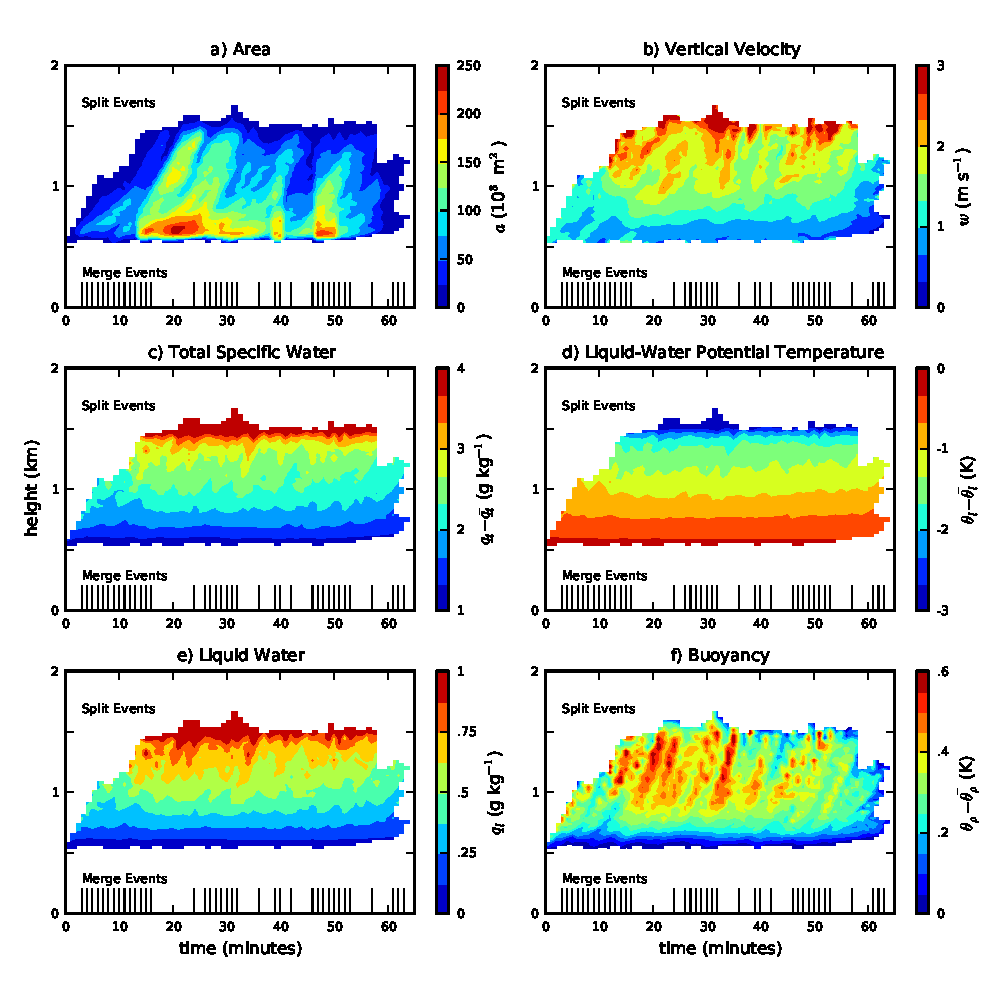
\includegraphics[width=\textwidth]{./figures/example_core}
\end{center}
\caption{As in as Figure \ref{fig:example_cloud}, but for the cloud core region.}
\label{fig:example_core}
\end{figure*}

%f
\begin{figure}[t]
\vspace*{2mm}
\begin{center}
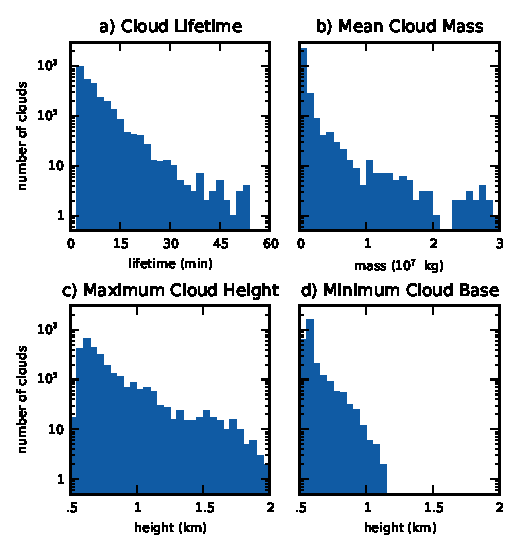
\includegraphics[width=8.3cm]{./figures/cloud_stats}
\end{center}
\caption{Bin-width normalized number densities ($n(x)dx$) of a) cloud lifetime 
in minutes (with a 2 minute bin width), b) mean mass of the cloud condensed 
region over the cloud lifetime (10$^6$ kg bin width), c) maximum height reached 
by the cloud top (50 m bin width), and d) minimum height of the cloud base 
(50 m bin width) for tracked clouds with complete life histories.}
\label{fig:cloud_stats}
\end{figure}

%f
\begin{figure}[t]
\vspace*{2mm}
\begin{center}
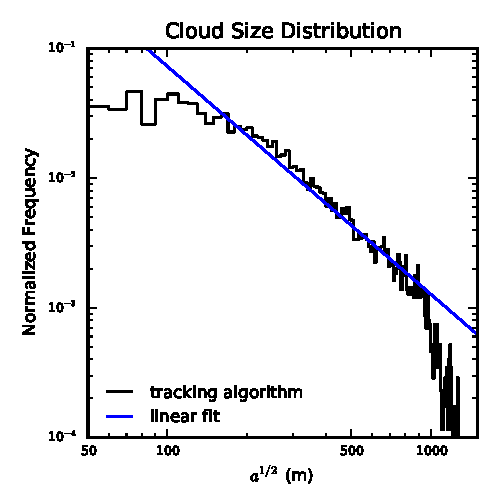
\includegraphics[width=8.3cm]{./figures/cloud_areas}
\end{center}
\caption{Histograms of horizontal cloud length scales calculated from 
instantaneous cloud field snapshots (black line) and from the cloud tracking 
algorithm (grey line) using a 10 m bin width. The red dashed line and blue 
dotted line show linear best fit between 100-1,000 m length scales to the 
instantaneous and tracked cloud histograms, respectively.}
\label{fig:cloud_areas}
\end{figure}

%f
\begin{figure*}[t]
\vspace*{2mm}
\begin{center}
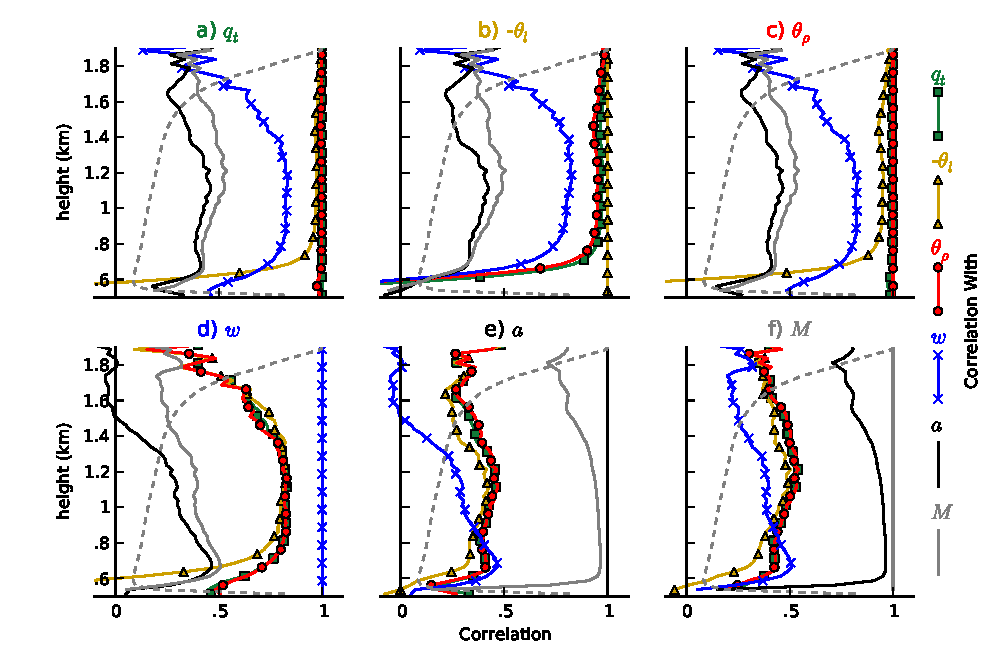
\includegraphics[width=\textwidth]{./figures/cloud_autocorrelation}
\end{center}
\caption{Vertical profiles of cross-correlations between condensed region 
a) mean total specific water $q_t$, b) mean liquid-water potential 
temperature $\theta_l$, c) mean density potential temperature $\theta_\rho$, 
d) mean vertical velocity $w$, e) horizontal cross-sectional area $a$ and 
d) vertical mass flux $M$.  Green squares denote correlations with $q_t$, 
yellow triangles correlations with -$\theta_l$, red circles correlations with 
$\theta_\rho$, blue x markers correlations with $w$, unmarked black lines 
correlations with $a$, and unmarked grey lines correlations with $M$. The 
dashed line denotes the 99\% confidence level for the correlation to be 
significantly different than zero.}
\label{fig:cloud_autocorrelation}
\end{figure*}

%f
\begin{figure*}[t]
\vspace*{2mm}
\begin{center}
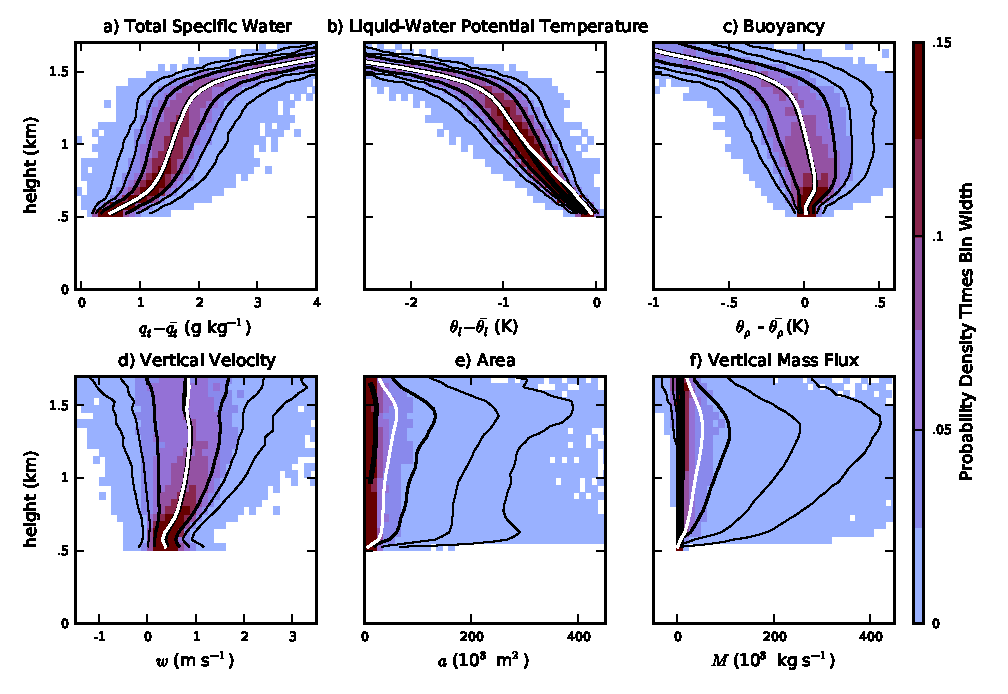
\includegraphics[width=\textwidth]{./figures/mean_profiles}
\end{center}
\caption{Variation with height of the bin-width normalized probability 
density functions ($P(x) \Delta x$) of a) mean total specific water excess, 
b) mean liquid-water potential temperature deficit, c) mean buoyancy, d) mean 
vertical velocity, e) horizontal cross-sectional area, and f) vertical mass 
flux of the condensed liquid-water regions of the tracked clouds.  Black lines 
show contours of the cumulative distribution functions of each variable at the 
0.01, 0.05, 0.16, 0.5, 0.84, 0.95, and 0.99 levels, from left to right.  White 
line denotes the mean values for each variable. }
\label{fig:mean_profiles}
\end{figure*}

%f
\begin{figure*}[t]
\vspace*{2mm}
\begin{center}
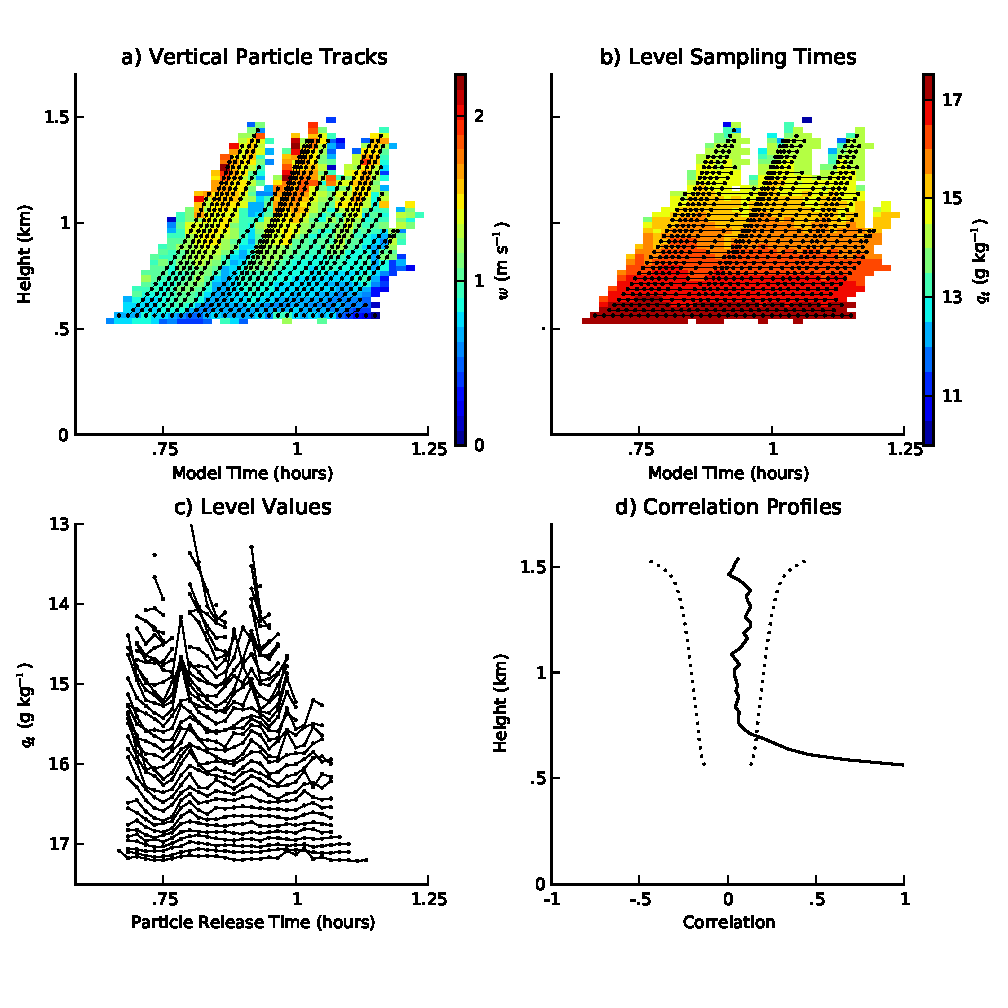
\includegraphics[width=\textwidth]{./figures/cloud_base_schematic}
\end{center}
\caption{Method used to determine correlations between lower- and upper-level 
cloud properties. a) Numerical particles are released once per minute from an 
initial level in the cloud and advected vertically with the mean vertical 
velocity of the cloud until the particle leaves the cloud. (Lines show the 
time-height trajectories of the numerical particles and colours show the 
cloud's vertical velocity.) b) The times at which particles reach each model 
level are then identified and the cloud properties at those times are recorded. 
(Dots show the time each particle reaches each model level and colours
show the cloud's vertical velocity. Only half the model levels have been 
plotted for clarity.)  c) The properties encountered by the particles at a 
given height are then arranged by the time each particle was released, forming 
a set of pseudo-time series at each height. (Dotted lines show the total 
specific water values of the cloud at the time each particle reached a given 
height.  The 600 m, 800 m, 1000 m, 1200 m, and 1400 m height particle values 
are highlighted and labeled.  Only half the model levels have been plotted.)  
d) Correlations are then taken between the properties of the particles at 
release and the properties at higher levels to calculate correlation profiles. 
(Solid line shows the correlation between total specific humidity of the 
particles at release and the total specific humidity of the cloud at various
heights. Dotted lines show the 99\% confidence level for a correlation to be
significantly different than zero.)}
\label{fig:cloud_base_schematic}
\end{figure*}

%f
\begin{figure}[t]
\vspace*{2mm}
\begin{center}
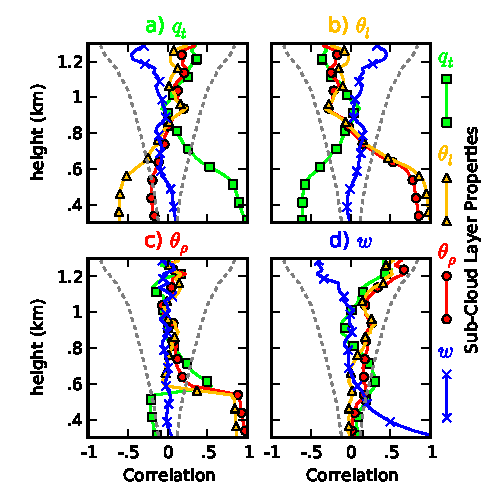
\includegraphics[width=8.3cm]{./figures/sub_cloud_profiles}
\end{center}
\caption{Correlation profiles between cloud plume properties near the middle 
of the sub-cloud layer at 300 m height and at higher levels for a) total 
specific water $q_t$, b) liquid-water potential temperature $\theta_l$, 
c) density potential temperature $\theta_\rho$, and d) vertical velocity $w$. 
Green squares show correlations with 300 m level $q_t$, yellow triangles 
correlations with 300 m $\theta_l$, red circles correlations with 300 m 
$\theta_\rho$, and blue x markers correlations with 300 m $w$.  Dotted lines 
show the 99\% confidence level for a correlation to be significantly different 
than zero.}
\label{fig:sub_cloud_profiles}
\end{figure}

%f
\begin{figure*}[t]
\vspace*{2mm}
\begin{center}
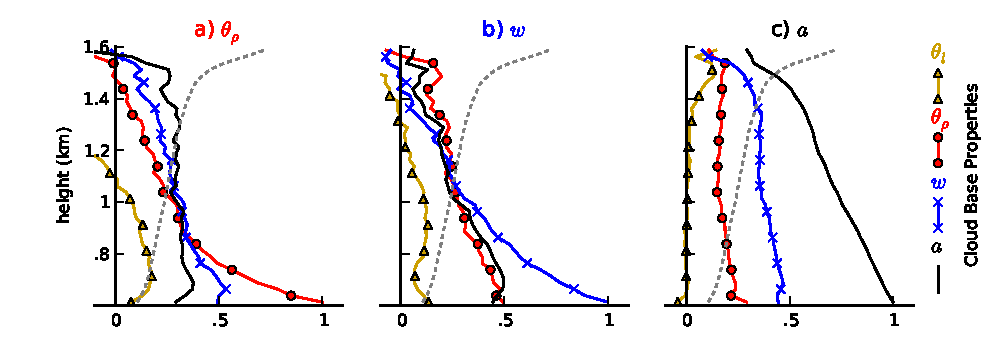
\includegraphics[width=\textwidth]{./figures/cloud_base_profiles}
\end{center}
\caption{Correlation profiles between cloud base properties at 600 m and 
at higher levels for a) density potential temperature $\theta_\rho$, b) 
vertical velocity $w$, and c) horizontal cross-sectional area $a$.  Yellow 
triangles show correlations with cloud base $\theta_l$, red circles show 
correlations with cloud base $\theta_\rho$, blue x markers correlations with 
cloud base $w$, and the black line show correlations with cloud base $a$. 
Dotted lines show the 99\% confidence level for a correlation to be 
significantly different than zero.}
\label{fig:cloud_base_profiles}
\end{figure*}

%f
\begin{figure*}[t]
\vspace*{2mm}
\begin{center}
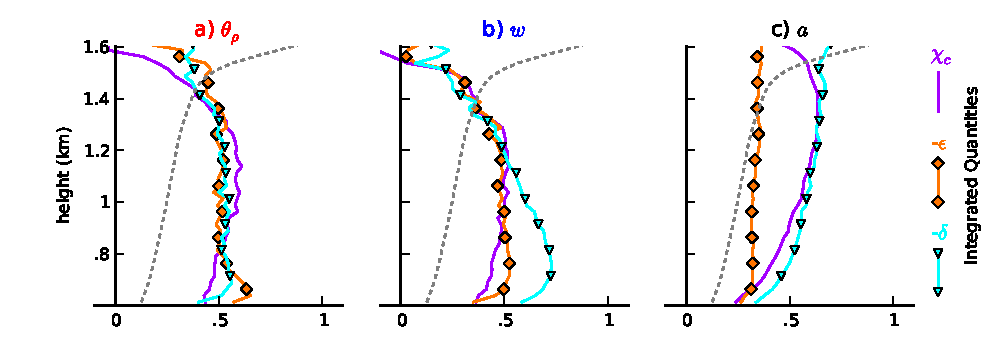
\includegraphics[width=\textwidth]{./figures/cloud_base_integrals_env}
\end{center}
\caption{Correlation profiles between cloud properties at each level and the 
mean of the entrainment/detrainment variables from cloud base at 600 m to the 
current level for a) density potential temperature $\theta_\rho$, b) 
vertical velocity $w$, and c) horizontal cross-sectional area $a$.  Yellow 
triangles show correlations with mean critical mixing fraction $\bar{\chi_c}$, 
orange diamonds show correlations with the negative of the mean fractional 
entrainment rate $\bar{\epsilon}$, and cyan triangles show correlations with 
the negative of the mean fractional detrainment rate $\bar{\delta}$.  Dotted 
lines show the 99\% confidence level for a correlation to be significantly 
different than zero.}
\label{fig:cloud_base_integrals_env}
\end{figure*}

%f
\begin{figure*}[t]
\vspace*{2mm}
\begin{center}
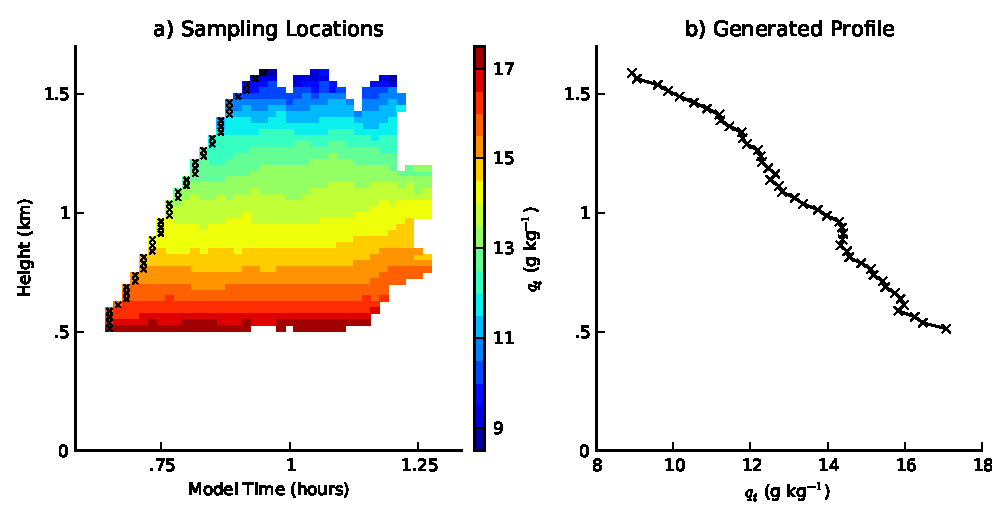
\includegraphics[width=\textwidth]{./figures/cloud_environment_schematic}
\end{center}
\caption{Method used to generate profiles of environmental properties 
encountered by a cloud during its initial ascent.  a) At each height, the 
earliest time the cloud is present is used to sample the mean properties of 
environmental points directly adjacent to the cloud, and the mean cloud points. 
b) These samples are used to generate a profile of the initial properties 
encountered by the cloud top.}
\label{fig:cloud_environment_schematic}
\end{figure*}

%f
\begin{figure*}[t]
\vspace*{2mm}
\begin{center}
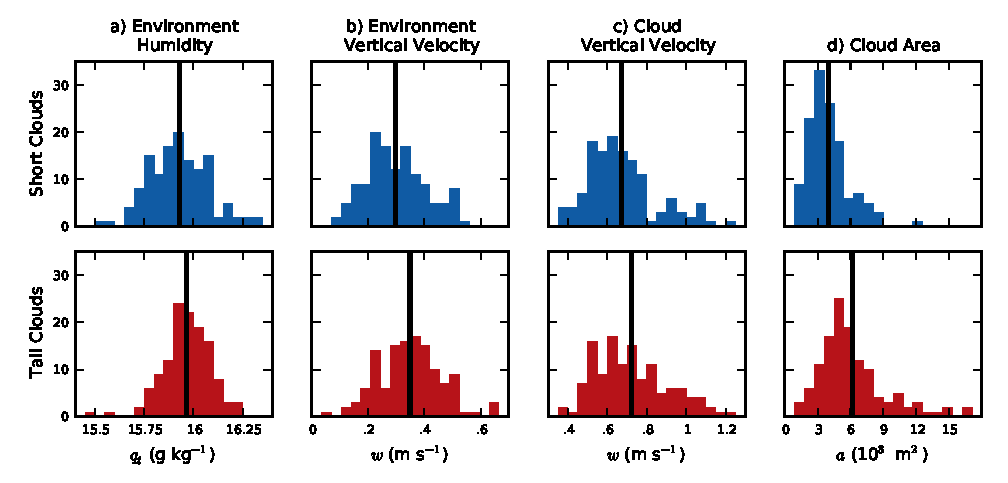
\includegraphics[width=\textwidth]{./figures/cloud_environment_histograms}
\end{center}
\caption{Bin-width normalized probability density functions ($P(x)dx$) of 
mean properties between 550-750 m of a) environmental vertical velocity, 
b) cloud density potential temperature, c) cloud vertical velocity, and 
d) horizontal cloud cross-sectional area.  Top row, blue histograms show clouds 
with maximum height less than 1,150 m; bottom row, red histograms show clouds 
with maximum height greater than 1,150 m.  Black lines show mean value of each 
histogram.}
\label{fig:cloud_environment_histograms}
\end{figure*}

%f
\begin{figure}[t]
\vspace*{2mm}
\begin{center}
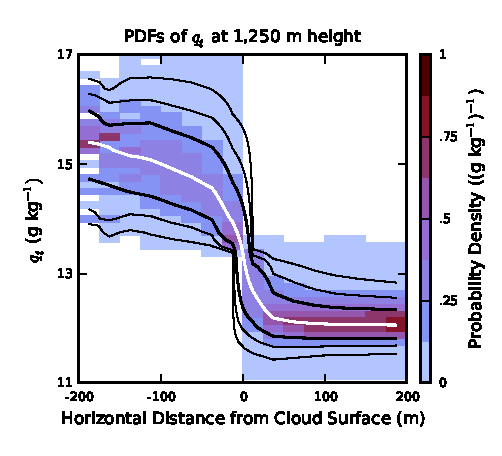
\includegraphics[width=8.3cm]{./figures/qt_vs_dist}
\end{center}
\caption{Variation in the probability density function of total specific 
water $q_t$ at 1,250 m height with distance from the nearest cloud surface.  
Probability density functions are taken at 25 m distance intervals, to match 
the model grid spacing.  Negative distances represent points inside the cloud.  
Black lines show contours of the cumulative distribution functions of each 
variables at the 0.01, 0.05, 0.16, 0.84, 0.95, and 0.99 levels, from bottom to 
top; white line shows the 0.5 level of the cumulative distribution function. 
Horizontal dotted line shows the domain-average specific humidity.}
\label{fig:qt_vs_dist}
\end{figure}

%% TABLES %%%%%%%%%%%%%%%%%%%%%%%%%%%%%%%%%%%%%%%%%%%%%%%%%%%%%%%%%%%%%%%%%%%%


%% ONE-COLUMN TABLE

%% TWO-COLUMN TABLE

%t
\begin{table*}[t]
\label{tbl:mannwhitneyu}
\caption{Mann-Whitney U-test results comparing differences between 
encountered environment and rising cloud top properties for tall vs short 
clouds.  For average properties between 550-750 m, tall clouds are defined as 
clouds that reach heights over 1,050 m; for average properties between 
750-1,000 m, tall clouds are those that reach heights over 1,300 m.  Shown are 
differences in the means (tall minus short), the differences in the means 
normalized by the standard deviation, the U-value, and the p-value that this 
U-value would arise for two samples taken from the same distribution. Variables 
with p-values \textless 0.05 (``possibly significant'') are shaded in light 
gray, and variables with p-values \textless 2.3 x 10$^{-3}$ (``definitely 
significant'') are shaded in darker gray.}
\vskip4mm
\centering
\begin{tabular}{lccccccc}
\tophline
& Variable & Number of & Number of & Mean difference & Mean difference  & Mann-Whitney & Mann-Whitney \\
& & tall clouds & short clouds & (tall minus short) & divided by variable  & U-value & p-value \\
& & & & & standard deviation & & \\

\middlehline
%-----------------------
environment 550-750 m & & 131 & 126 & & & & \\
& $q_t$       & & & 0.03 g kg$^{-1}$ &  0.14 & 7391  &  0.15 \\
& $\theta_l$ & & & -0.0015 K                   & -0.02 & 8167 & 0.89 \\
& $\theta_\rho$ & & & 0.004 K               & 0.09 & 7603.5  & 0.28    \\
\rowcolor[gray]{0.95}
& $w$         & & &  0.05 m s$^{-1}$         &  0.38 & 6450 & 2.5x10$^{-3}$ \\
\middlehline
%-----------------------
cloud 550-750 m & & & & & & \\
\rowcolor[gray]{0.85}
& $q_t$       & & &  0.031 g kg$^{-1}$         &  0.43 & 6044  & 2.1x10$^{-4}$ \\
\rowcolor[gray]{0.85}
& $q_l$       & & &  6.7x10$^{-3}$ g kg$^{-1}$ &  0.41 & 6386  & 1.7x10$^{-3}$  \\
& $\theta_l$ & & & -1.1x10$^{-3}$ K           & -0.05 & 8006  & 0.68 \\
\rowcolor[gray]{0.95}
& $\theta_\rho$ & & &  0.018 K               &  0.37 & 6450  & 2.5x10$^{-3}$ \\
\rowcolor[gray]{0.85}
& $w$         & & &  0.08 m s$^{-1}$           &  0.47 & 6039  & 2.0x10$^{-4}$ \\
\rowcolor[gray]{0.85}
& $a$         & & &  7748 m$^2$                &  0.95 & 3383 & 3.0x10$^{-16}$ \\
\rowcolor[gray]{0.85}
& $M$         & & &  6193 kg s$^{-1}$    &  1.04 & 2667 & 6.8x10$^{-21}$ \\
\middlehline
%-----------------------
environment 750-1000 m & & 127 & 113 & & & & \\
& $q_t$       & & &  0.018 g kg$^{-1}$         &  0.07 & 6893 & 0.60 \\
& $\theta_l$ & & & -0.008 K                   & -0.07 & 6932 & 0.65 \\
& $\theta_\rho$ & & & -3.5x10$^{-4}$ K       & -0.006 & 7028 & 0.78 \\
& $w$         & & &  0.03 m s$^{-1}$           &  0.17 & 6659 & 0.34 \\
\middlehline
%-----------------------
cloud 750-1000 m & & & & & &          \\
\rowcolor[gray]{0.85}
& $q_t$       & & &  0.17 g kg$^{-1}$        &  1.10 & 2544   & 6.3x10$^{-18}$ \\
\rowcolor[gray]{0.85}
& $q_l$       & & &  0.06 g kg$^{-1}$        &  1.05 & 2836   & 6.3x10$^{-16}$ \\
\rowcolor[gray]{0.85}
& $\theta_l$ & & & -0.05 K                  & -1.00 & 2921.5 & 2.1x10$^{-15}$  \\
\rowcolor[gray]{0.85}
& $\theta_\rho$ & & & 0.10 K                &  1.02 & 2918  & 2.1x10$^{-15}$ \\
\rowcolor[gray]{0.85}
& $w$         & & &  0.15 m s$^{-1}$         &  0.70 & 4212   & 3.4x10$^{-8}$  \\
\rowcolor[gray]{0.85}
& $a$         & & &  8100 m$^2$             &  1.07 & 2405 & 6.3x10$^{-19}$ \\
\rowcolor[gray]{0.85}
& $M$         & & &  11656 kg s$^{-1}$    &  1.11 & 1716 & 2.7x10$^{-24}$ \\
%-----------------------
\bottomhline
\end{tabular}
\end{table*}

%% The different columns must be separated with a & command and should
%% end with \\ to identify the column brake.

%%%%%%%%%%%%%%%%%%%%%%%%%%%%%%%%%%%%%%%%%%%%%%%%%%%%%%%%%%%%%%%%%%%%%%%%%%%%%%


%% If figures and tables must be numbered 1a, 1b, etc. the following command
%% should be inserted before the begin{} command.

%\addtocounter{figure}{-1}\renewcommand{\thefigure}{\arabic{figure}a}


\end{document}
